\section{Organization settings}
\label{sec:settings-feature-organization}

This page is your organization’s identity card in the system: its logos, colors, homepage images, address and defaults, plus the limits on attached files. Open it when you first set up the organization, then whenever its identity or details change. Its values affect every member, so its card appears in “Settings” for the organization owner only.

\begin{rcnote}[Example: Horizon]
The system administrator uploads the company logo at ①, chooses its color at ②, then writes the subdomain \en{hzn} and saves the page, so the logo and color appear for Sarah Al-Khatib and Omar Haddad when they sign in.
\end{rcnote}

\begin{figure}[H]
\centering
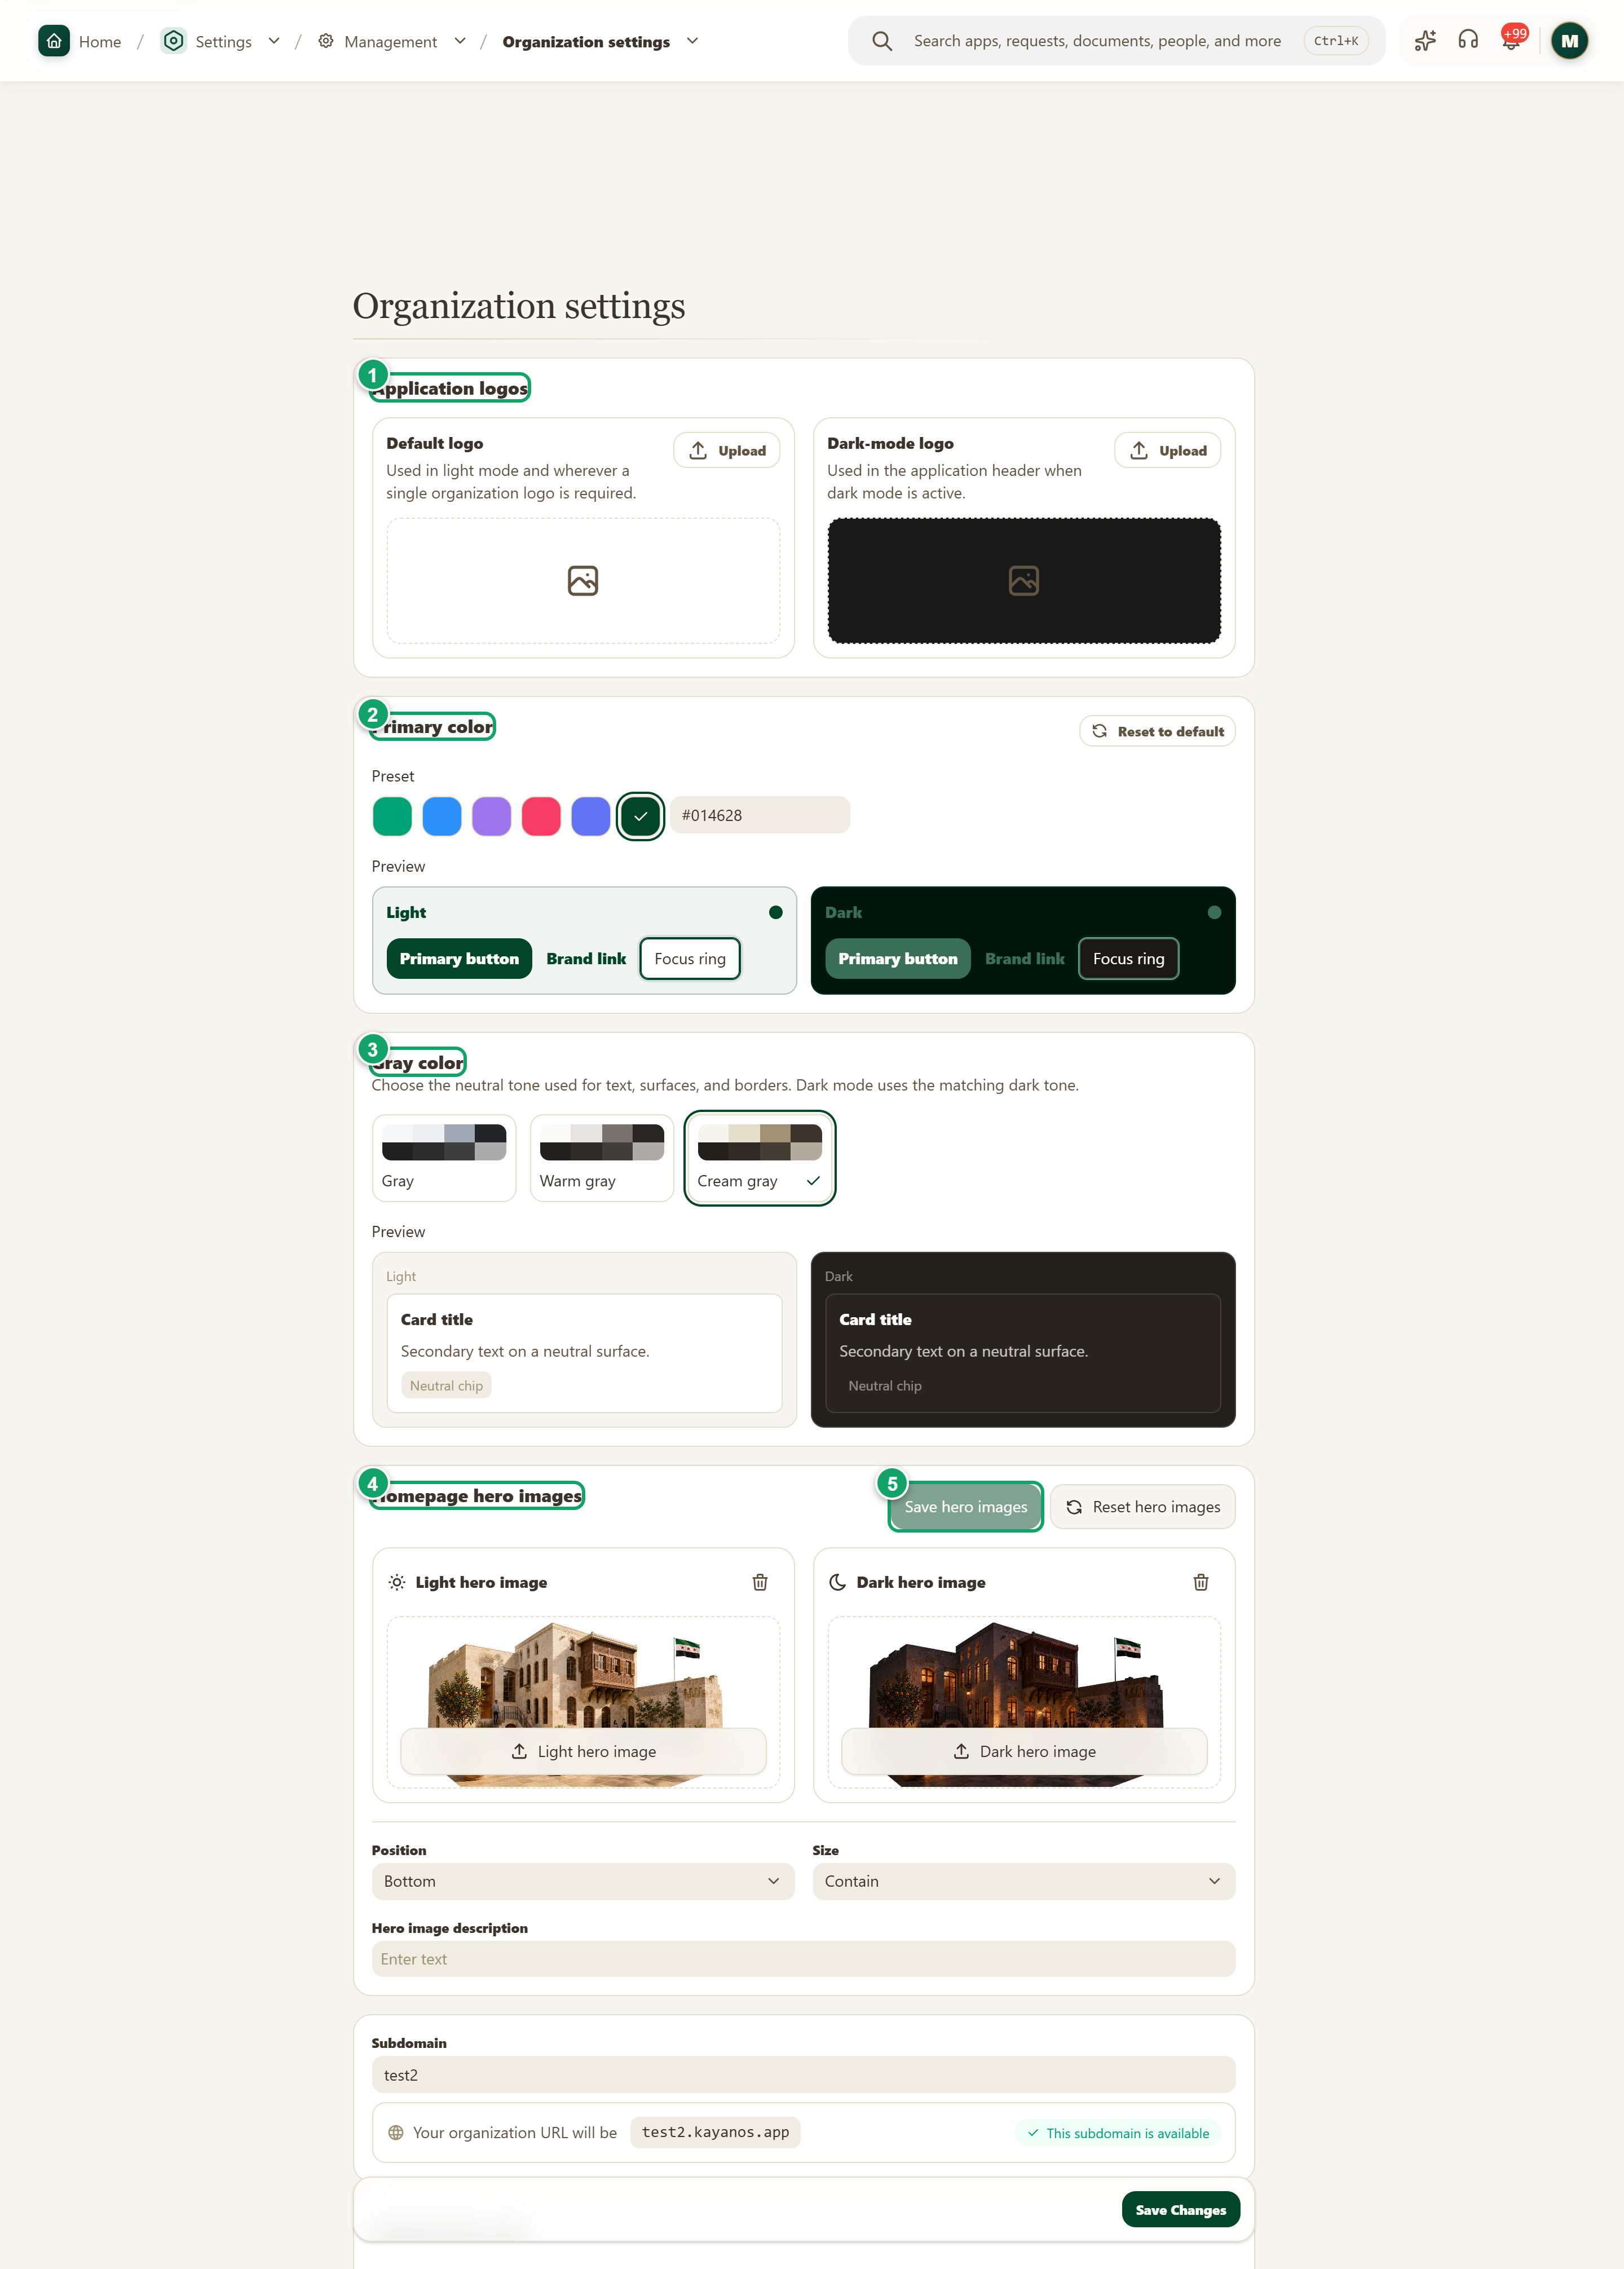
\includegraphics[width=0.95\linewidth,height=0.72\textheight,keepaspectratio]{figures/screens/ch08-organization-en.png}
\caption{The organization’s visual identity}
\label{fig:settings-organization-screen}
\shotnote{The image shows the visual part of the test organization’s page, where no logo has been uploaded yet. The preview cards show a color’s effect before saving, so try it there first; nothing reaches members until you save. ① “Application logos”: one logo for light mode and one for dark mode. ② “Primary color”: a preset or a custom color; “Reset to default” restores the original. ③ “Gray color”. ④ “Homepage hero images”: two images, for the light and dark appearance. ⑤ “Save hero images”: saves the images alone and stays disabled until you change something in them.}
\end{figure}

\begin{figure}[H]
\centering
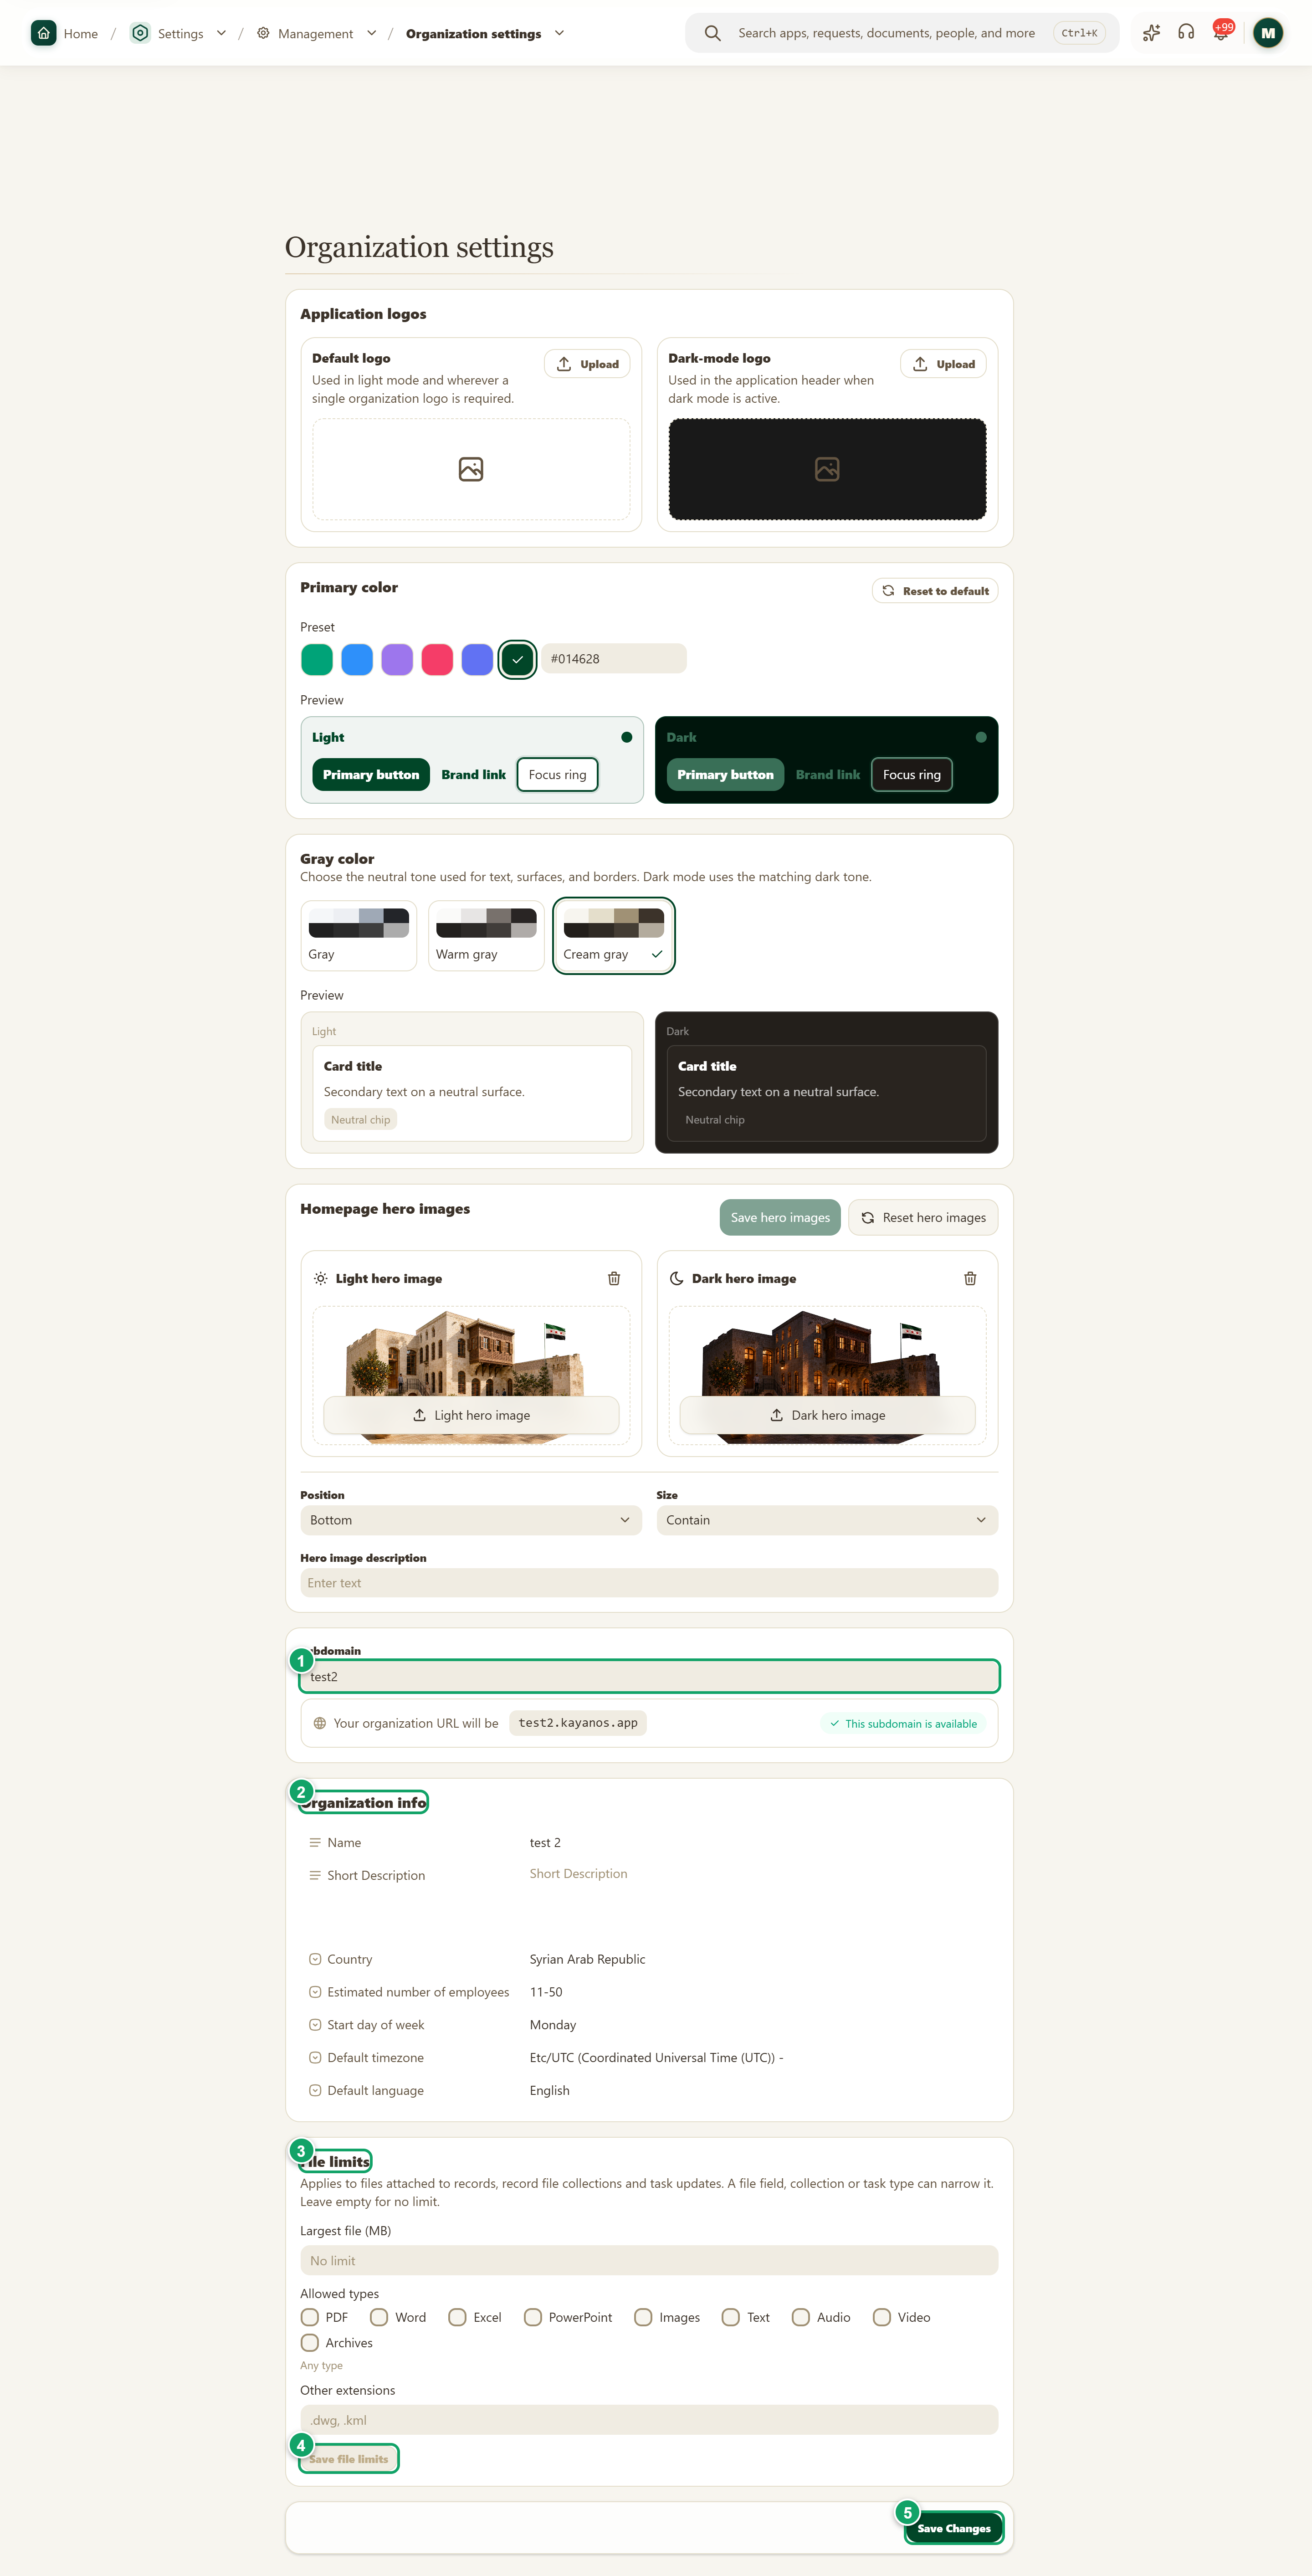
\includegraphics[width=0.95\linewidth,height=0.72\textheight,keepaspectratio]{figures/screens/ch08-organization-info-en.png}
\caption{Address, details and file limits}
\label{fig:settings-organization-info-screen}
\shotnote{The image shows the whole page with the test organization’s values, focusing on its lower part. These sections set the organization’s address and values other pages rely on. Note the two separate buttons: file limits do not save with the rest of the page. ① “Subdomain”: changing it changes the organization’s whole sign-in address. ② “Organization info”. ③ “File limits”. ④ “Save file limits”: saves this section alone. ⑤ “Save Changes”: saves the identity, subdomain, details and hero images.}
\end{figure}

\begin{table}[H]
\centering
\caption{What do you record in Organization settings?}
\label{tab:settings-organization-fields}
\begin{tabularx}{\linewidth}{R{4.2cm} Y}
\rcHeaderRow
\thh{Section or field} & \thh{What do you record?}\\
“Application logos” & “Default logo” for light mode and wherever a single logo is required, and “Dark-mode logo” for the application header in dark mode. Each takes an image up to 5 MB.\\
“Primary color” & The organization’s color on buttons and links. Pick a “Preset” or type a custom color code.\\
“Gray color” & The neutral tone for text, surfaces and borders: “Gray”, “Warm gray” or “Cream gray”.\\
“Homepage hero images” & One image per appearance, up to 5 MB, with “Position”, “Size” and “Hero image description” in each language.\\
“Subdomain” & The first part of your organization’s address. It takes lowercase Latin letters, digits and hyphens, 3 to 63 characters, and its availability is checked as you type.\\
“Name” and “Short Description” & The organization’s name and description in each language. The name is required in at least one language.\\
“Country” and “Estimated number of employees” & Two required descriptive details.\\
“Start day of week” & The day the week starts on in the calendar and timesheets.\\
“Default timezone” & The time the organization works by; export dates use it.\\
“Default language” & Chosen from the active languages, and used when a member has no preferred language.\\
“File limits” & “Largest file (MB)”, “Allowed types” and “Other extensions” for files attached to records and task updates. Leave the section empty for no limit; a file field or task type can narrow it.\\
\end{tabularx}
\end{table}

\begin{enumerate}
\item In “Settings”, open “Organization settings”.
\item Upload the logos with “Upload”, then pick the primary and gray colors and review the two previews.
\item Change the hero images if you need to, then review “Subdomain” until “This subdomain is available” appears.
\item Complete “Organization info”, then press “Save Changes”.
\item If you changed the file limits, press their own button, “Save file limits”.
\end{enumerate}

\textbf{Check:} A success message appears after saving, the new values are there when you reopen the page, and “Saved” appears beside the file limits button. If you changed the subdomain, the browser moves you to the new address, so tell your members.

\clearpage
\section{Notification defaults}
\label{sec:settings-feature-notifications}

This page sets which channels work by default for each kind of notification, so members need not adjust dozens of options themselves. Use it when you start with the system, or when the team complains of too many of one notification or of missing important ones. It appears for the organization owner and anyone allowed to edit roles. A member can still change their own choices under “Notification settings” in their account.

\begin{rcnote}[Example: Horizon]
The system administrator goes to the “Tasks” group, turns on Email for “Task assigned” at ④, then presses “Save” at ⑤. From then on Omar Haddad gets this notification by email unless he changes his choice in his account.
\end{rcnote}

\begin{figure}[H]
\centering
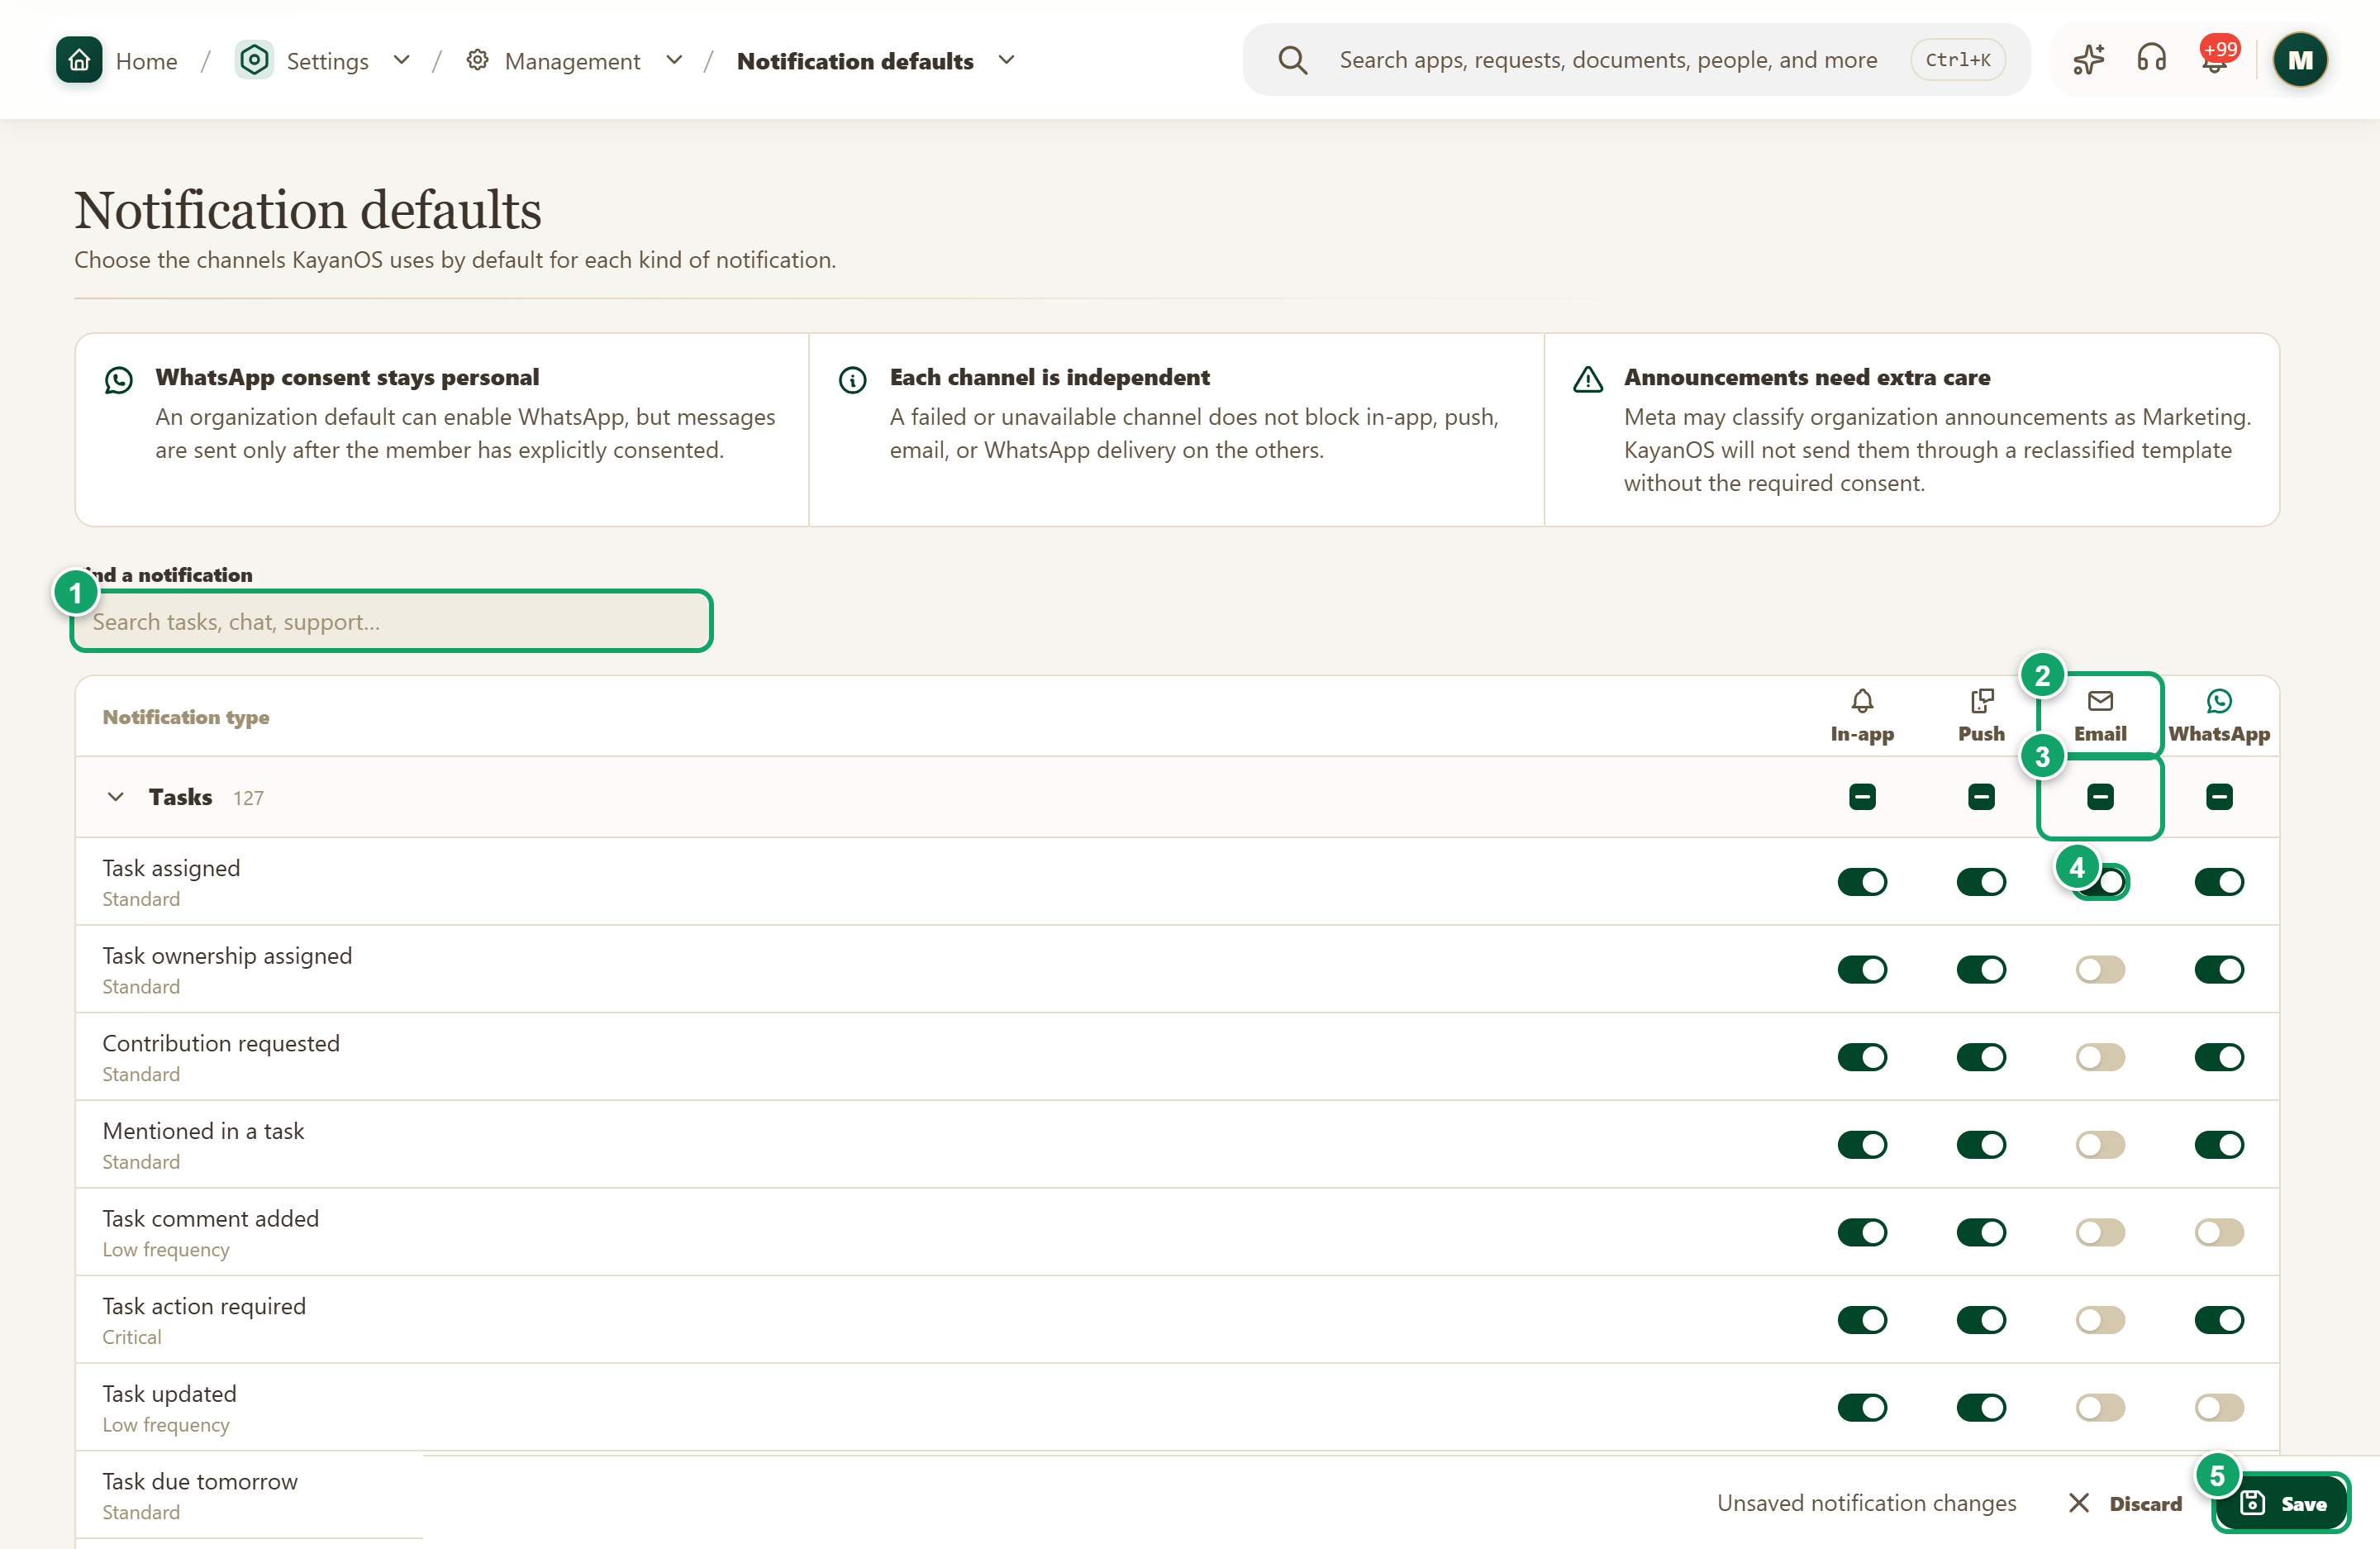
\includegraphics[width=0.95\linewidth,height=0.72\textheight,keepaspectratio]{figures/screens/ch08-notifications-en.png}
\caption{The notification table with one unsaved change}
\label{fig:settings-notifications-screen}
\shotnote{The image shows rows of the “Tasks” group in the test organization; one switch was changed to bring up the save bar, and the change was then discarded. Rows are kinds of notification, columns are the channels, and nothing applies before you save. ① “Find a notification”: it currently searches internal English names, not the names you see. ② The “Email” column. ③ The group box: it applies a value to that channel in all the group’s rows; a dash inside it means mixed values. ④ The channel switch for one kind of notification. ⑤ “Save”: appears with “Discard” after the first change.}
\end{figure}

\begin{table}[H]
\centering
\caption{What do you record in Notification defaults?}
\label{tab:settings-notifications-fields}
\begin{tabularx}{\linewidth}{R{4.2cm} Y}
\rcHeaderRow
\thh{Item} & \thh{What does it mean?}\\
“In-app” & A notification in the system’s notification list.\\
“Push” & An alert sent to the member’s device.\\
“Email” & A message to the member’s email address.\\
“WhatsApp” & A WhatsApp message, sent only after the member has explicitly consented, even if the organization turns it on.\\
Groups & Notifications by source: “Tasks”, “Chat”, “Calendar”, “Email”, “System”, “Support \& SLA”, “Signing”, “Attendance” and “Official correspondence”.\\
Notification level & Shown under its name: “Low frequency”, “Standard”, “Urgent” or “Critical”. It is fixed information you do not change here.\\
Empty cell & A channel not available for this kind of notification, so it has no switch.\\
\end{tabularx}
\end{table}

\begin{figure}[H]
\centering
\begin{tikzpicture}[node distance=0.5cm]
\node[stepBox] (a) {The member’s own choice, if any};
\node[stepBox,below=of a] (b) {The organization’s setting on this page, if any};
\node[stepBox,below=of b] (c) {The system’s original value};
\draw[flowsTo] (a) -- (b);
\draw[flowsTo] (b) -- (c);
\end{tikzpicture}
\rclegend
\caption{Which value applies to a member?}
\label{fig:settings-notifications-order}
\shotnote{The system starts from the member’s choice; if there is none it moves to the organization’s setting, then to the original value. So saving this page does not change what a member chose personally. If a member misses a notification the organization turned on, check their own choices first.}
\end{figure}

\begin{enumerate}
\item In “Settings”, open “Notification defaults” and read the three notes at the top.
\item Go to the group you want; it is the surest way to a notification, because the search box does not find visible names yet.
\item Change the channel switch for one kind, or use the group box to change all its rows.
\item Press “Save”, or “Discard” to drop your changes.
\end{enumerate}

\textbf{Check:} The “Unsaved notification changes” bar disappears after saving, and the switches keep their new values when you reopen the page. If “These defaults changed elsewhere” appears, someone else saved first; press “Reload” and review the values.

\clearpage
\section{Export jobs}
\label{sec:settings-feature-export-jobs}

This page creates a copy of the organization’s data as a ZIP file holding one Excel file per record type; the page calls record types “Entities”. Use it when you need a copy for archiving, audit or analysis outside the system. Only the organization owner can open it, because the files carry the organization’s data; keep them somewhere safe after downloading.

\begin{rcnote}[Example: Horizon]
The system administrator is Horizon’s organization owner. He presses “New export” at ①, chooses the last quarter’s records, returns when the status is “Completed” at ③, and downloads the file at ⑤ before it expires.
\end{rcnote}

\begin{figure}[H]
\centering
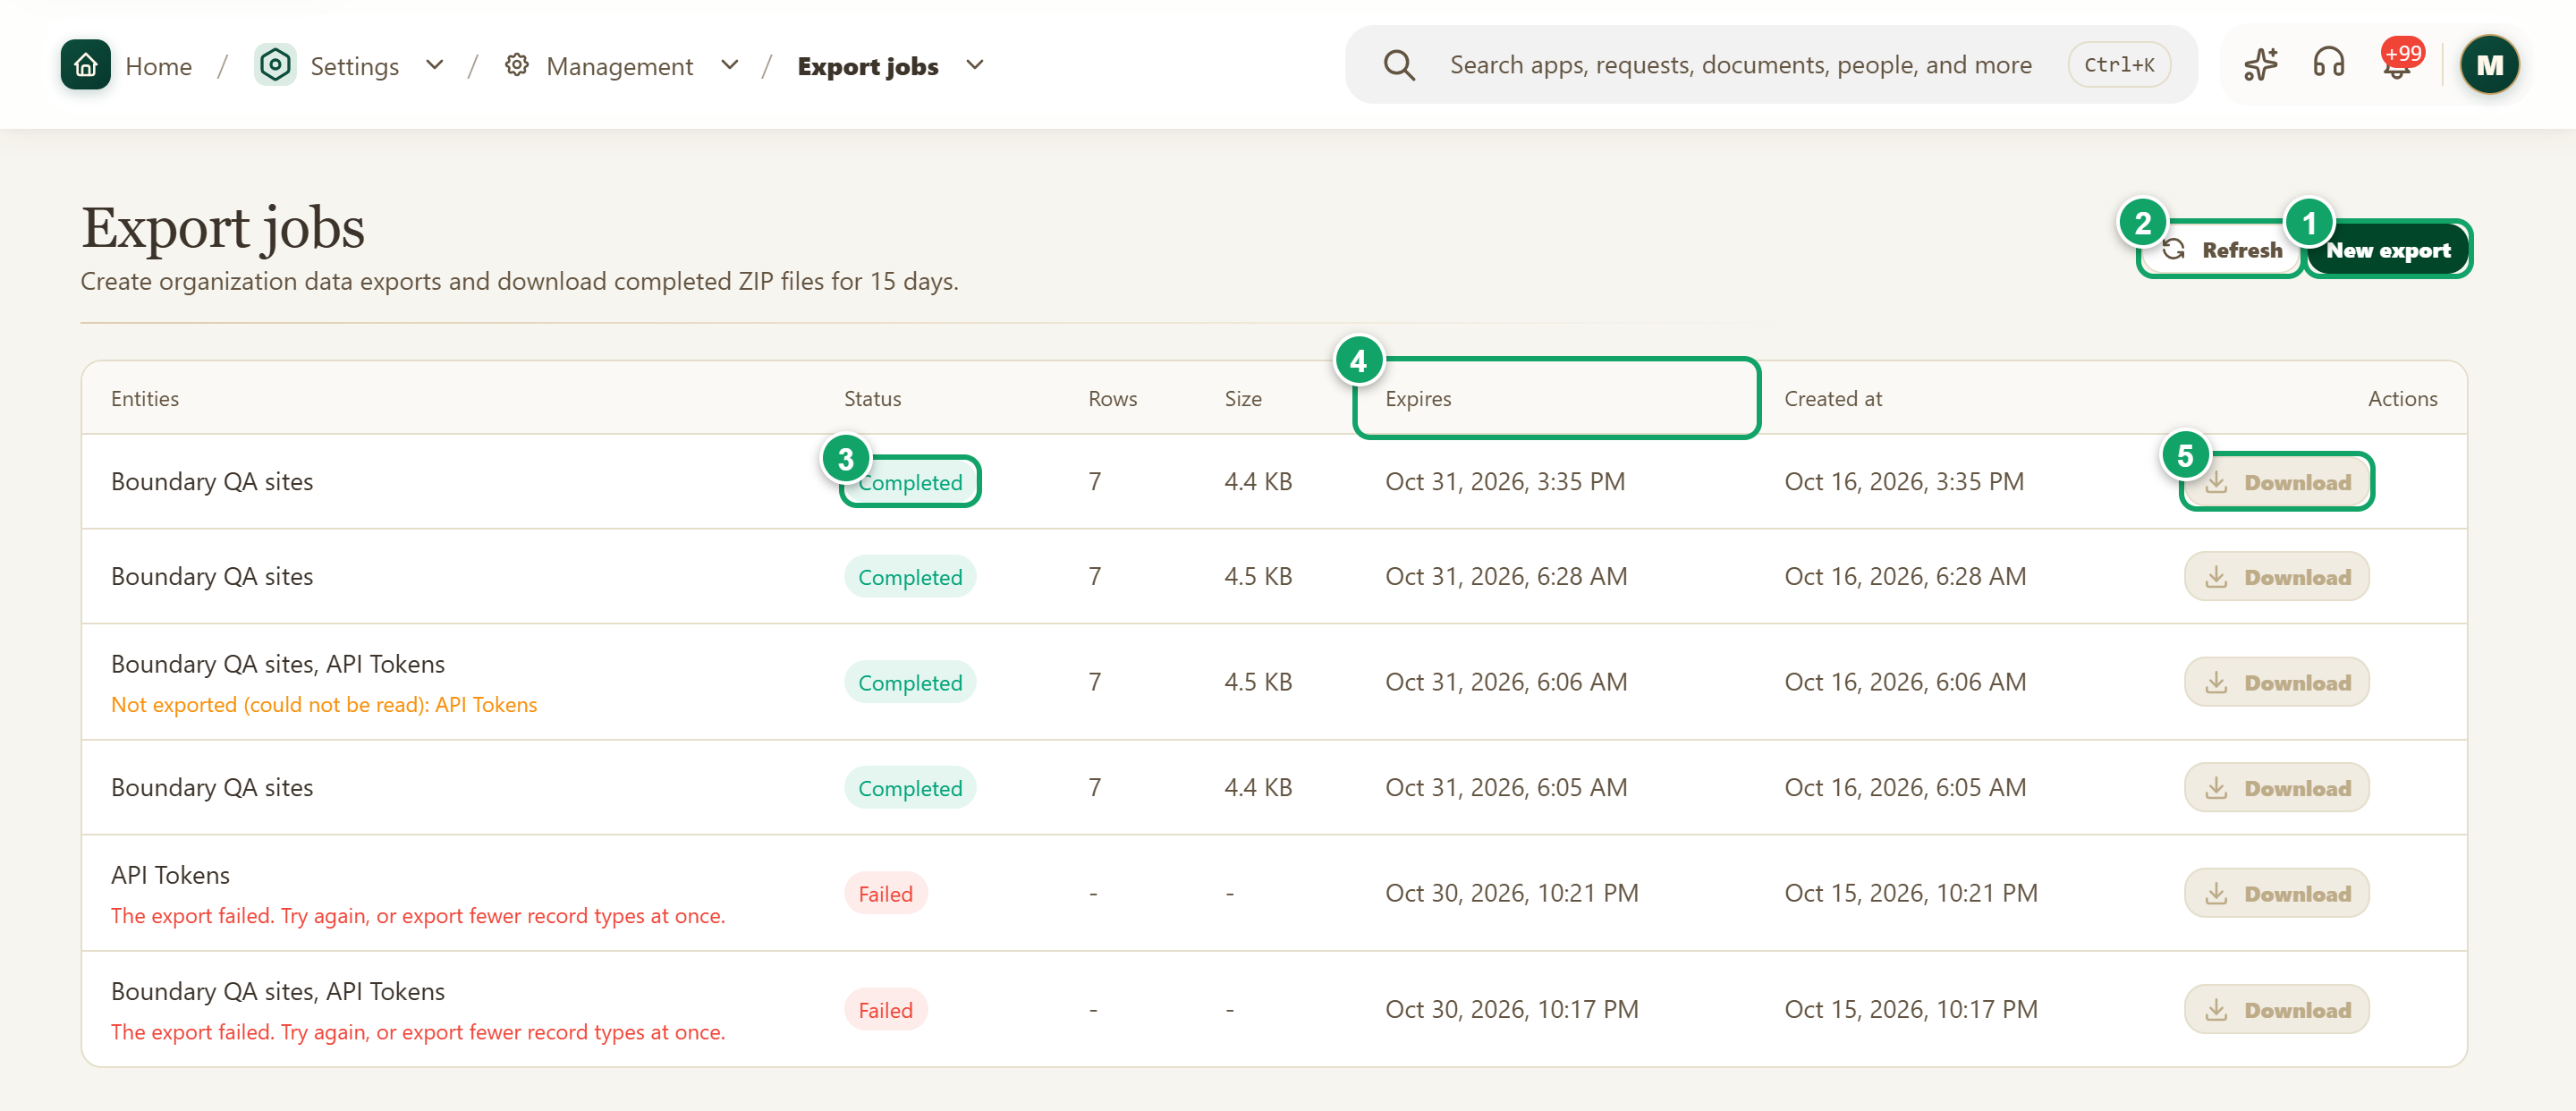
\includegraphics[width=0.95\linewidth,height=0.72\textheight,keepaspectratio]{figures/screens/ch08-export-jobs-en.png}
\caption{The list of export jobs}
\label{fig:settings-export-jobs-screen}
\shotnote{The image shows earlier test jobs whose time has passed, which is why every “Download” button is disabled. The list records each export the organization requested, with its status, size and the date downloads stop. ① “New export”. ② “Refresh”: rereads the list, which also updates by itself every ten seconds while a job runs. ③ Status: “Pending”, then “Processing”, then “Completed” or “Failed”. ④ “Expires”: the last moment to download, 15 days after creation. ⑤ “Download”.}
\end{figure}

\begin{figure}[H]
\centering
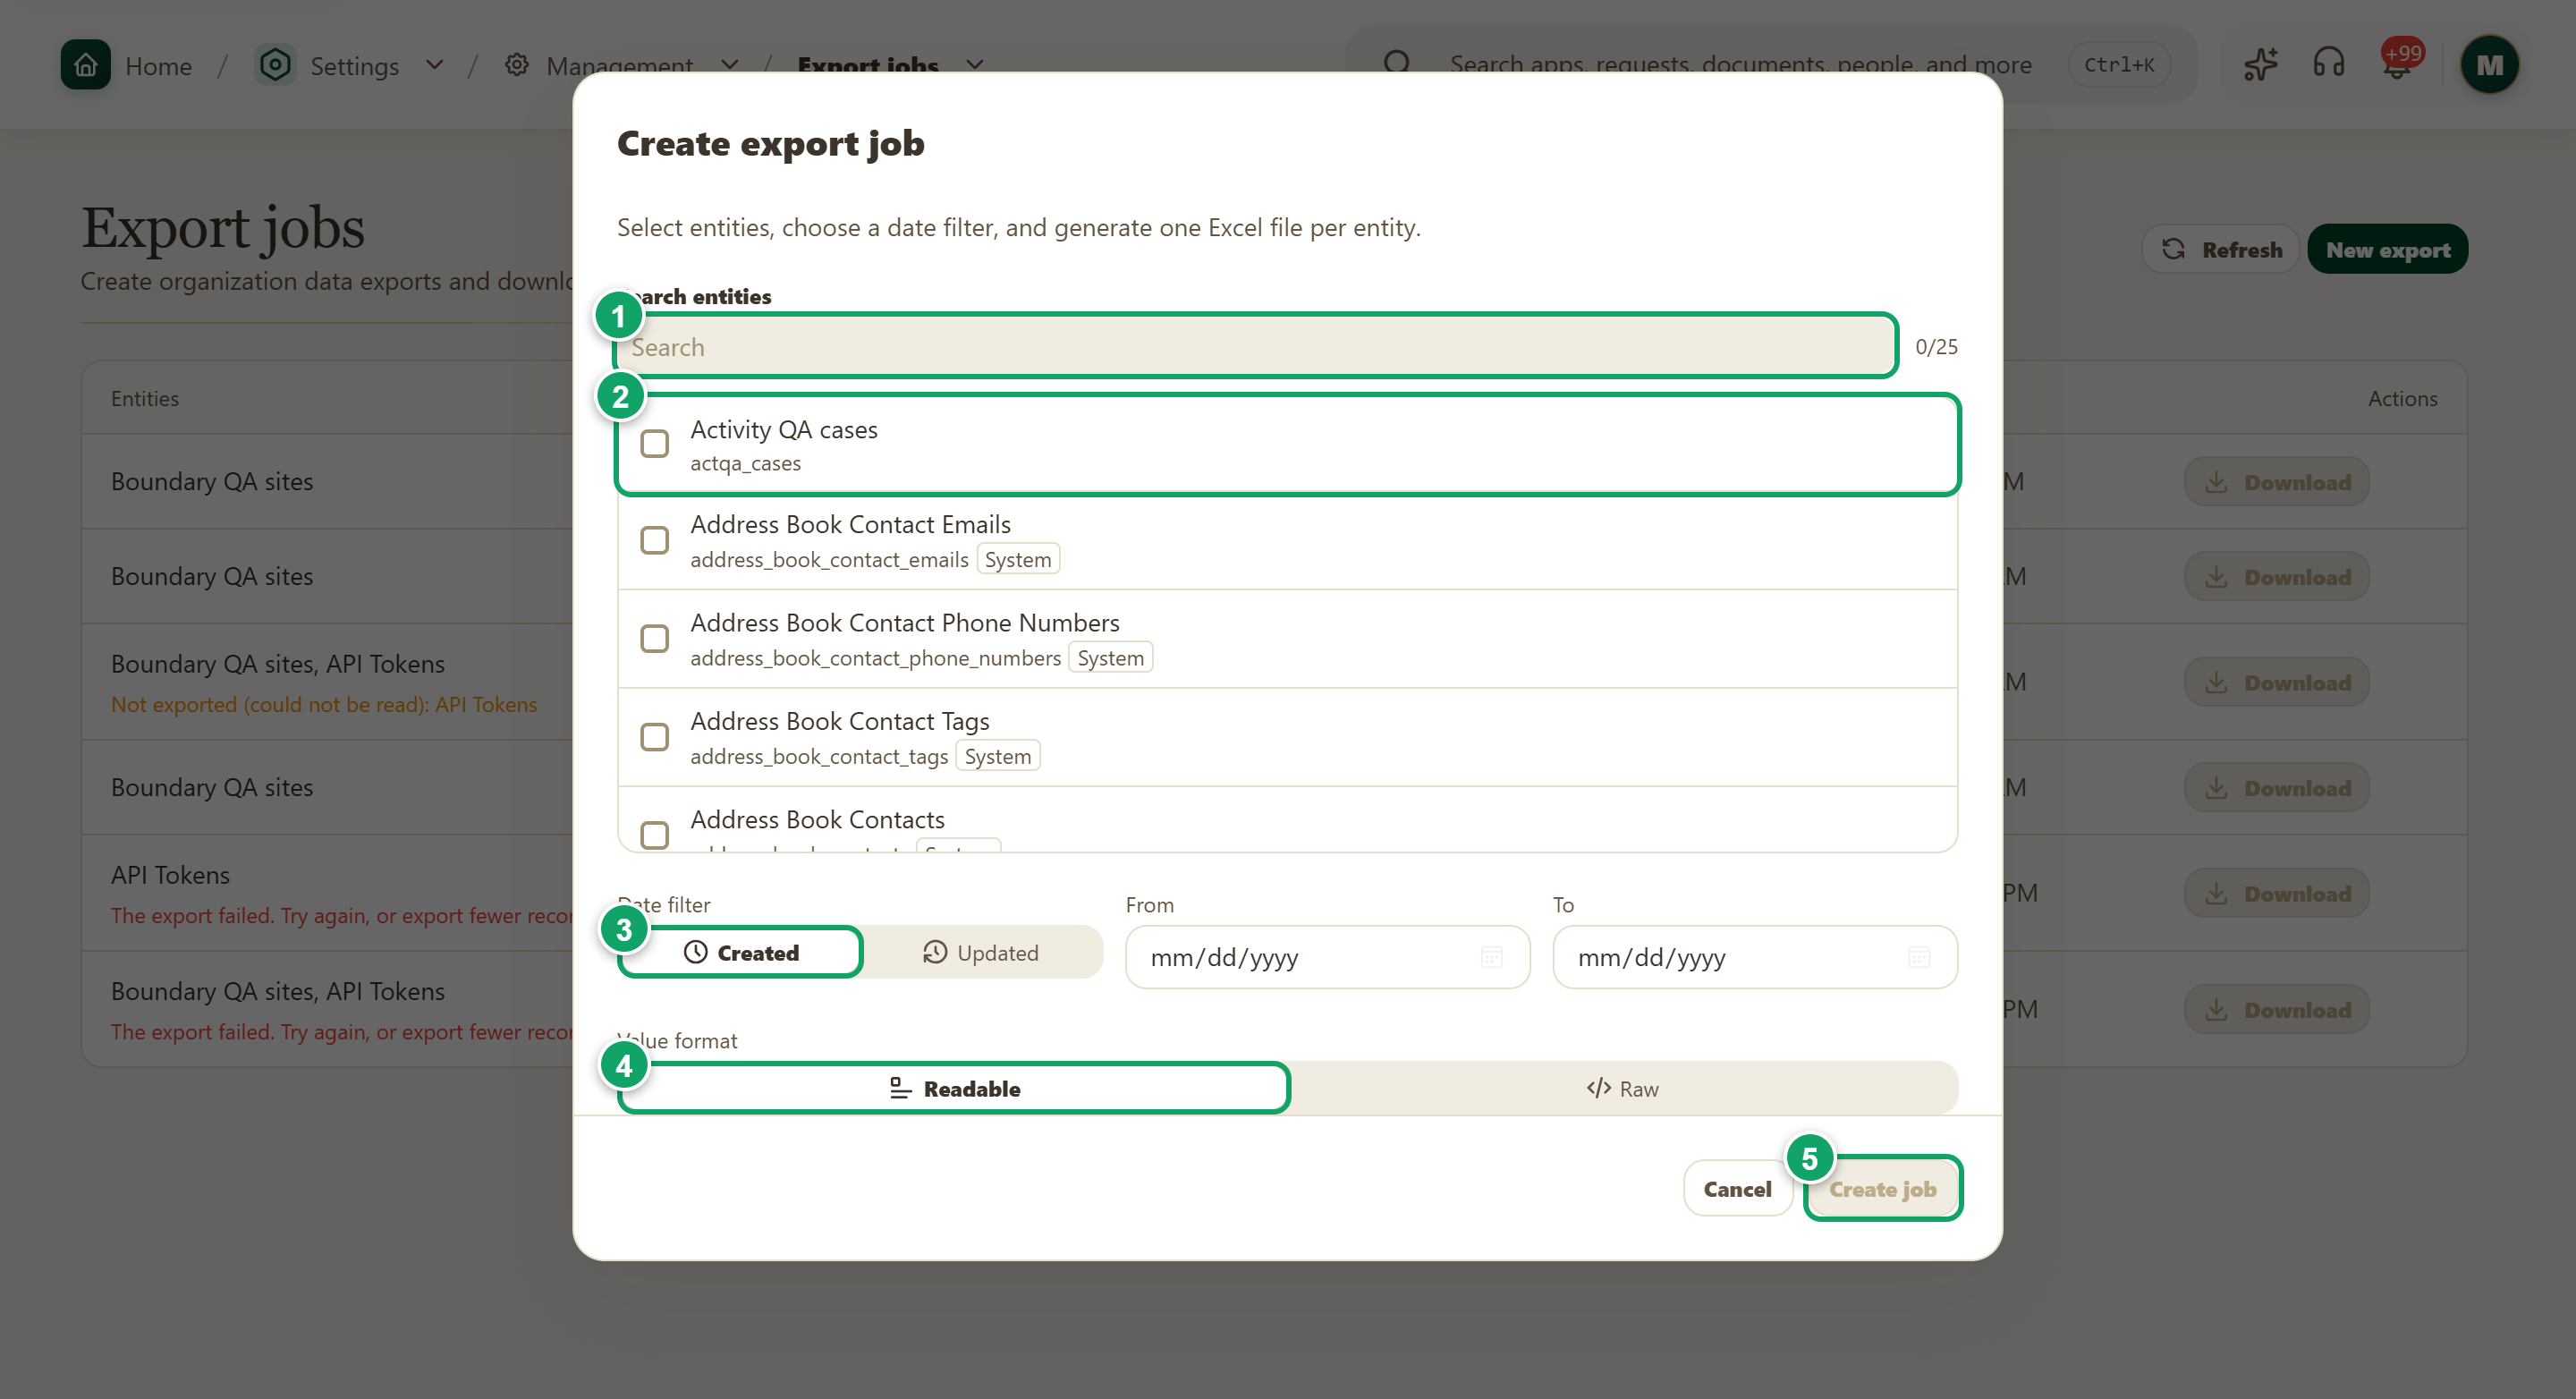
\includegraphics[width=0.95\linewidth,height=0.72\textheight,keepaspectratio]{figures/screens/ch08-export-jobs-create-en.png}
\caption{The Create export job window}
\label{fig:settings-export-jobs-create-screen}
\shotnote{The image shows the window before anything is chosen, so the create button stays disabled and the names are the test organization’s. Your choices here decide what goes into the file and how its values appear. The window was closed without creating a job. ① “Search entities”, beside a counter of selected types out of 25. ② A record type, selected by pressing it; it may carry a “System” or “Native” tag. ③ “Date filter”. ④ “Value format”. ⑤ “Create job”.}
\end{figure}

\begin{table}[H]
\centering
\caption{What do you record in an export job?}
\label{tab:settings-export-jobs-fields}
\begin{tabularx}{\linewidth}{R{4.2cm} Y}
\rcHeaderRow
\thh{Field} & \thh{What do you record?}\\
Entities & The record types you want, up to 25 in one job.\\
“Date filter” & Whether the period is measured on the record’s “Created” or “Updated” date.\\
“From” and “To” & The limits of the period, both optional. The start date must not come after the end date.\\
“Value format” & “Readable” shows values as staff understand them; “Raw” shows them as stored in the system.\\
\end{tabularx}
\end{table}

\begin{enumerate}
\item In “Settings”, open “Export jobs”, then press “New export”.
\item Search for the record types and select them, then choose the “Date filter” and period if you want part of the data.
\item Choose “Readable” for direct reading, or “Raw” if the file will move to another system.
\item Press “Create job”, wait until the status is “Completed”, then press “Download”.
\end{enumerate}

\textbf{Check:} The job appears in the list, and “Download” becomes available when it completes. No more than two jobs run at once in an organization. If “Not exported (too many rows, choose a shorter date range)” appears under the name, that type passed 100,000 records, so export it again with a shorter period. If a job shows “Failed”, try again with fewer types.

\clearpage
\section{Reports}
\label{sec:settings-feature-reports}

This page gathers the values every report starts with: periods, currency view, how reports are sent and kept, and keyboard keys. A report designer therefore need not repeat these decisions, and cannot send a report through a channel the organization does not allow. The page carries a “Beta” tag and appears for the organization owner and holders of the Administrator role, who alone can change its values.

\begin{rcnote}[Example: Horizon]
The system administrator keeps “Secure link” at ③ and “E-mail” allowed, leaves WhatsApp off, then presses “Save” at ⑤. When Omar Haddad prepares his monthly report, the WhatsApp channel is not available to him.
\end{rcnote}

\begin{figure}[H]
\centering
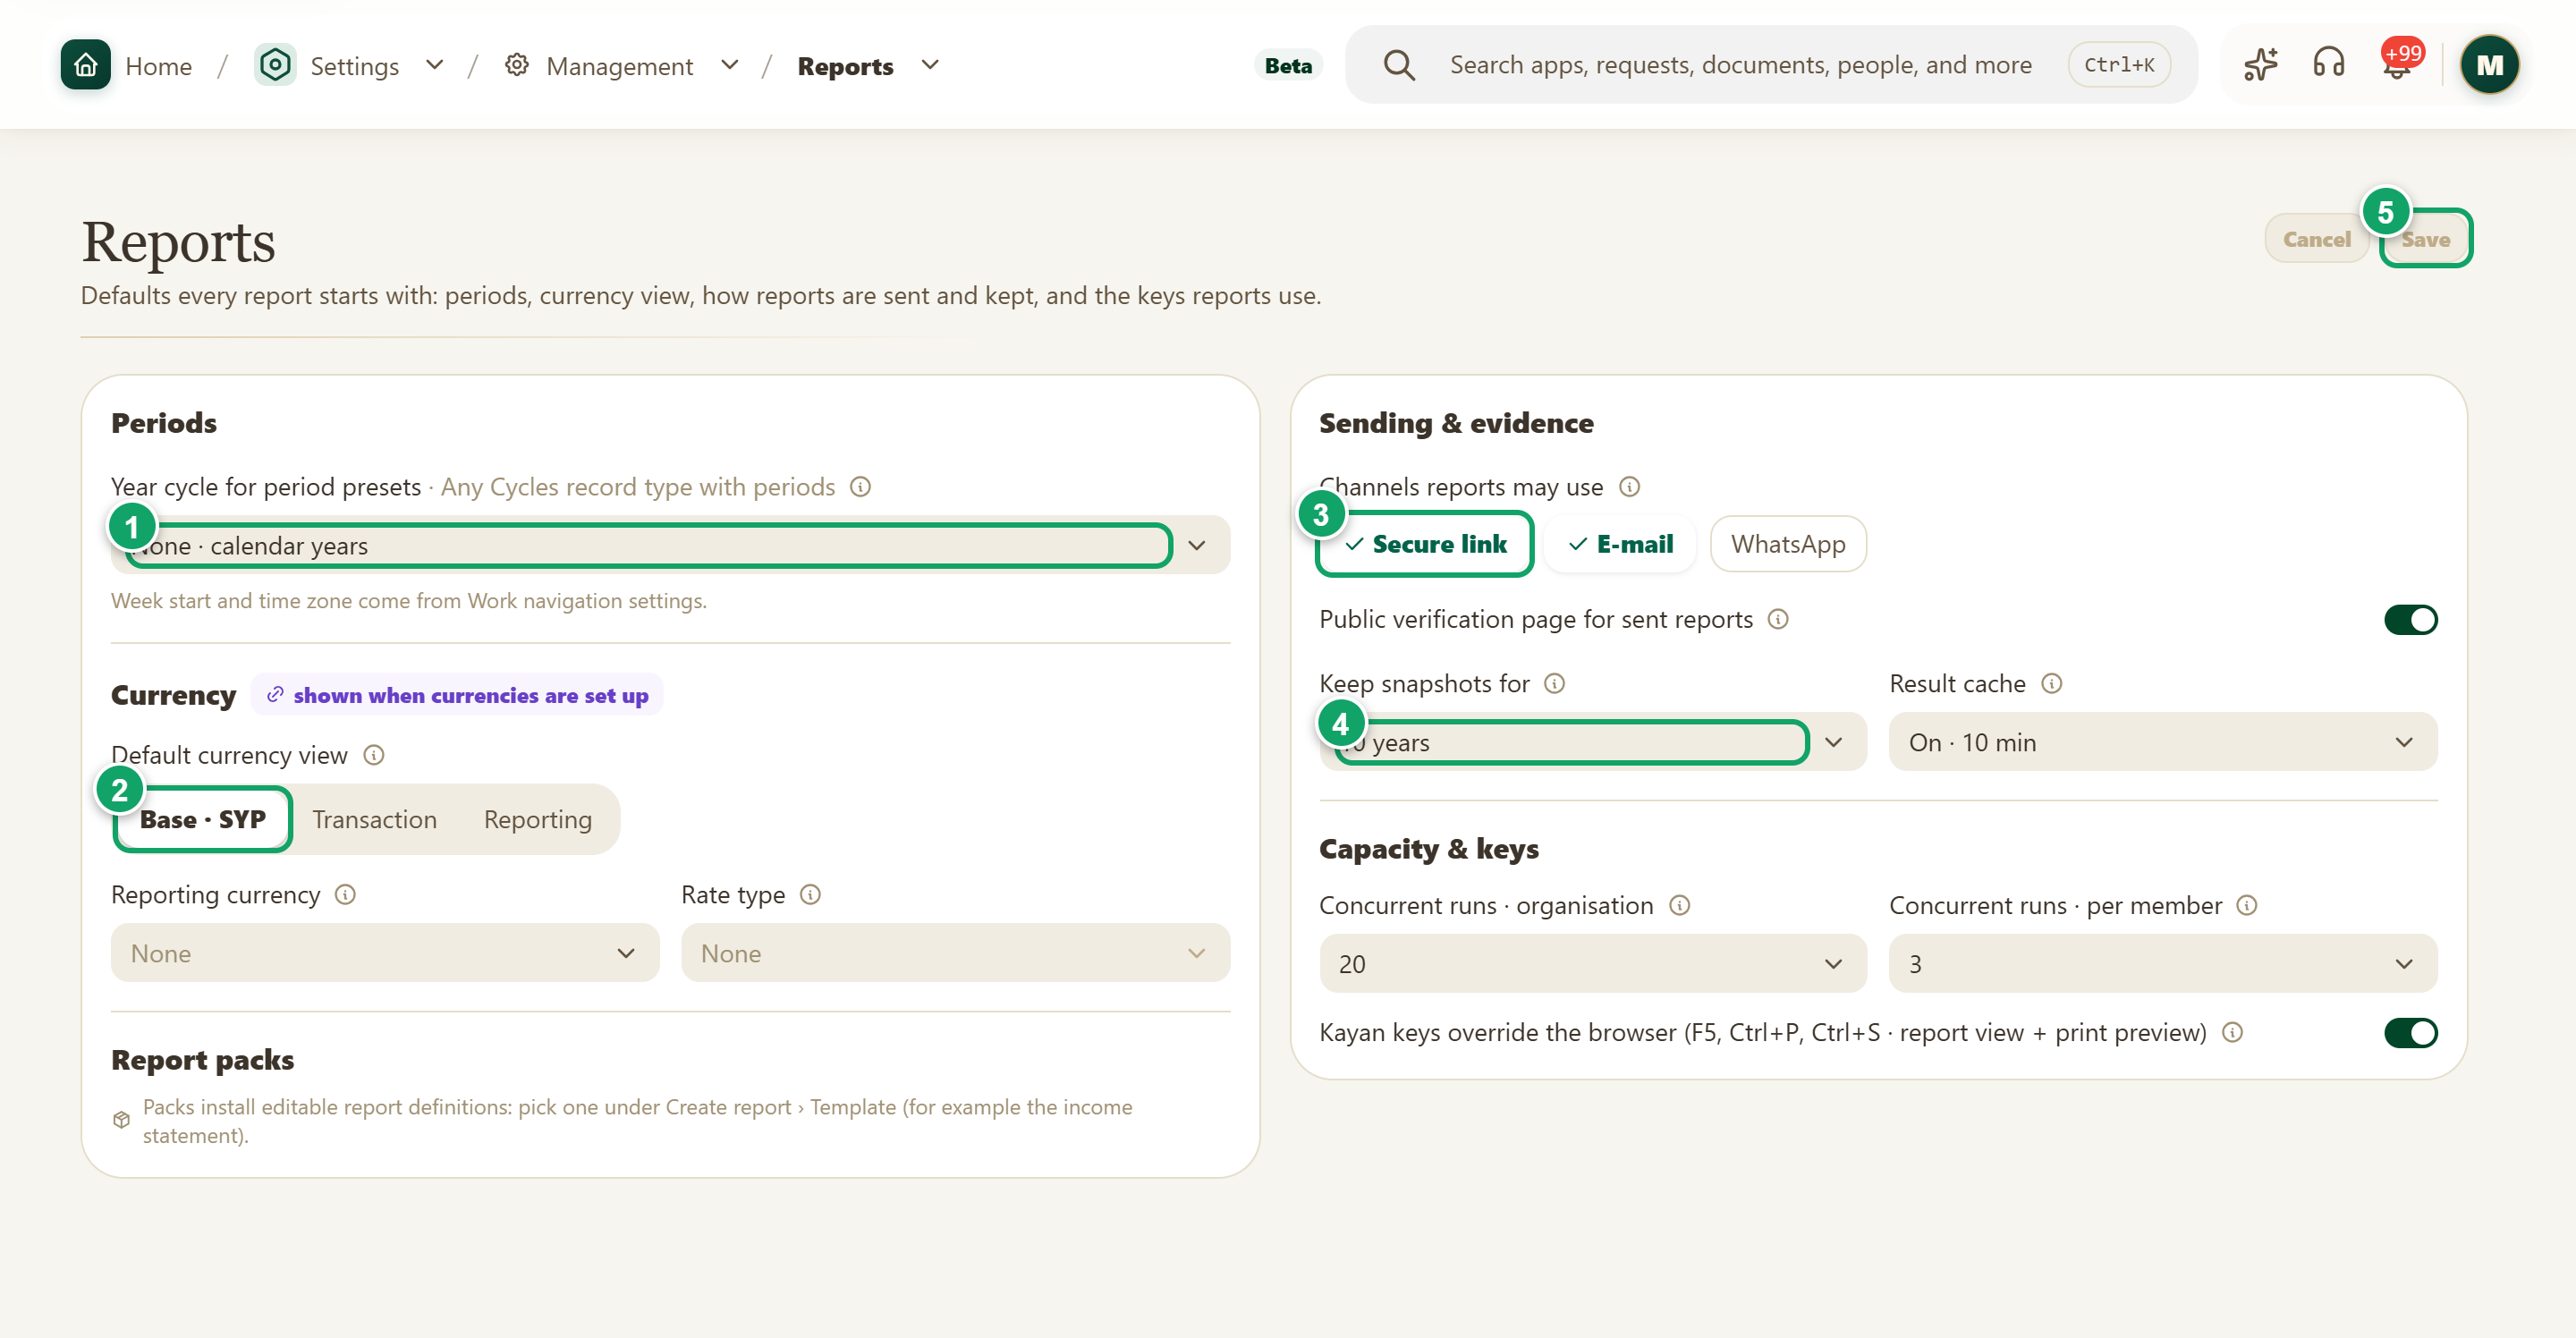
\includegraphics[width=0.95\linewidth,height=0.72\textheight,keepaspectratio]{figures/screens/ch08-reports-en.png}
\caption{Report settings}
\label{fig:settings-reports-screen}
\shotnote{The image shows the test organization’s values; its base currency is \en{SYP}. These values apply to all reports. The channels matter most, because turning one off blocks it in every report. Week start and time zone for periods come from “Work navigation settings”, not this page. ① “Year cycle for period presets”: the current value is calendar years. ② “Default currency view”. ③ “Channels reports may use”: press a channel to turn it on or off. ④ “Keep snapshots for”. ⑤ “Save”: becomes available with “Cancel” after the first change.}
\end{figure}

\begin{table}[H]
\centering
\caption{What do you record in Reports settings?}
\label{tab:settings-reports-fields}
\begin{tabularx}{\linewidth}{R{4.2cm} Y}
\rcHeaderRow
\thh{Field} & \thh{What do you record?}\\
“Year cycle for period presets” & The Cycles record type whose periods define “This year”, “Year to date” and “This period”. Without it, calendar years are used.\\
“Default currency view” & “Base”, “Transaction”, meaning each line’s currency, or “Reporting”, the converted currency.\\
“Reporting currency” and “Rate type” & The currency amounts convert to and the rate used. If a rate is missing, the report stops with a clear message.\\
“Report packs” & A note that needs no input: packs are installed from “Create report › Template”.\\
“Channels reports may use” & “Secure link”, “E-mail” and “WhatsApp”.\\
“Public verification page for sent reports” & A sent copy carries a link and QR code to a page showing that its figures came from you and have not changed.\\
“Keep snapshots for” & How long fixed copies of reports are kept, from 1 to 20 years.\\
“Result cache” & Keeps a result for up to an hour so reopening it is quicker, or choose “Off”. Any new posting clears the kept result.\\
“Concurrent runs” & How many reports run at once: 5 to 50 for the organization and 1 to 5 per member; the rest wait their turn.\\
“Kayan keys override the browser” & In the report and print preview, \en{F5} refreshes the report, \en{Ctrl+P} prints it and \en{Ctrl+S} saves its options, instead of the browser acting.\\
\end{tabularx}
\end{table}

\begin{enumerate}
\item In “Settings”, open “Reports”, then review “Periods”.
\item Choose the currency view. If you choose “Reporting”, set the currency and rate type.
\item Set the allowed channels, verification page, retention and result cache.
\item Review “Capacity \& keys”, then press “Save”, or “Cancel” to return to the saved values.
\end{enumerate}

\textbf{Check:} “Report settings saved.” appears and both buttons are disabled until the next change. When a report is sent, a channel you turned off does not work. If another member opens the page by its link, they see “Only owners and administrators can change report settings.” and the fields are disabled.
